\documentclass{article}
\usepackage{fullpage}
\usepackage{graphicx}
\usepackage{hyperref}
\usepackage[usenames,dvipsnames]{color}
\usepackage{amssymb}
\usepackage{amsmath}
\usepackage{comment}
\usepackage[utf8]{inputenc}
\usepackage[T1]{fontenc}
\usepackage{listings}
\usepackage[finnish]{babel}
\usepackage{float}

\addtolength{\parskip}{\baselineskip}

\begin{document}

\title{
A13-10 Radio-ohjattavan pienoismallin ohjausjärjestelmän ja käyttöliittymän kehittäminen \\
AS-0.3200 Automaatio- ja systeemitekniikan projektityöt
}

\author{Toni Liski, Konsta Hölttä, Lasse Kortetjärvi}
\date{30.9.2013}

\maketitle

\section{Projektin tavoite}
\subsection{Tausta}

Projektin taustana on Aalto-yliopiston Insinööritieteiden korkeakoulun Koneenrakennustekniikan kurssi: Kon-16.4081 Ajoneuvojen tuotekehitys. Kurssilla aloitettiin vuonna 2011 projekti, jonka tarkoituksena oli rakentaa radio-ohjattavan auton pienoismalli ajodynamiikan opetuskäyttöön. Syksyllä 2012 Automaatio- ja systeemitekniikan projektityökurssilla autoon tehtiin osaprojektina Matlab-käyttöliittymä ja rakennettiin ohjelmisto ABS- ja ESP-ohjauksille. Molemmat projektit jäivät kuitenkin kesken, ja nyt niille on tekeillä jatkoprojekti sekä mekaniikan että mekatroniikan kannalta. Kon-16.4081-kurssin projektiryhmässä on tällä hetkellä viisi henkilöä jatkamassa heidän kesken jäänyttä projektiaan, ja Automaatio- ja systeemitekniikan projektityökurssilla puolestaan kolme henkilöä.

\subsection{Tehtävä}

Projektin tehtävänä on kehittää yllämainittuun kauko-ohjattavaan autoon toimivat lukkiutumattomien jarrujen (ABS) ja ajoneuvonhallintajärjestelmän (ESP) ohjaukset, kehittää auton käyttöliittymää ja toteuttaa automaattiohjaus etukäteen määriteltyjen reittipisteiden avulla. Lisäksi autoon lisätään etäisyysanturit helpottamaan paikoitusta testialustalla, eli tässä tapauksessa juoksumatolla. Samoja antureita hyödynnetään myös ennaltaehkäisemään ajoneuvon törmäyksiä kiinteisiin kohteisiin. Jos projektissa jää aikaa, toteutetaan kauko-ohjaus esimerkiksi RC-autosta tuttua kauko-ohjainta käyttäen, sekä käytetään etäisyysantureita automatisoimaan kulku seinää tai monimutkaista rataa vasten.
\subsection{Rajaus}

Projekti rajataan ohjaus- ja säätöjärjestelmien kehitykseen, käyttöliittymäkoodin parantamiseen ja muutamien testausta helpottavien antureiden lisäämiseen. Pyrimme minimaalisiin muutoksiin valmiissa komponenteissa ja elektroniikassa.

\subsection{Tavoite}

Tavoitteena on projektin lopuksi päästä testaamaan autoa eri ympäristöissä siten, että auton ohjelmisto ja säätöjärjestelmät ovat täysin kunnossa ja helposti jatkokehitettävissä. Tavoitteena on myös auton helppo kauko-ohjaus joko Matlab-käyttöliittymän kautta näppäimistön avulla, tai erillisellä kauko-ohjaimella tai joystickillä.

\subsection{Työryhmä}

Projektin toteuttavat Automaatio- ja Systeemitekniikan laitokselta Toni Liski, Konsta Hölttä ja Lasse Kortetjärvi.

\subsection{Ajankäyttö}

Projektin ajankäyttösuunnitelma esitetään luvussa 4: Ajankäyttö.

\section{Projektin lähtökohta}

\subsection{Yleiskuva}

Pienoismalli eli auton runko on vielä kehityksen alla ja siitä työstää tällä hetkellä viisihenkinen mekaniikkaryhmä. Autoon ollaan suunnittelemassa koria ja auton voimansiirto vaihdetaan akselivetoisesta hihnavetoiseksi. Mekaniikkaryhmän puolesta autolla päästään ajamaan aikaisintaan projektin loppuvaiheilla, kun uusi voimansiirto on toiminnassa. Auton ulkonäkö selviää kuvista \ref{fig:autoylhaalta} ja \ref{fig:autoedesta}.

\begin{figure}[p]
\centering
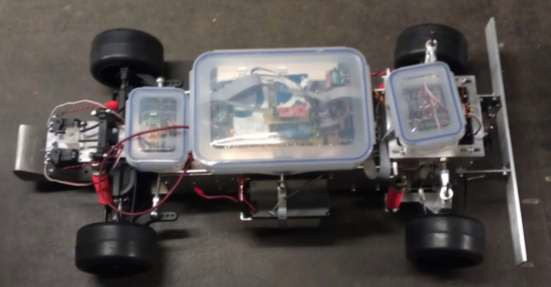
\includegraphics[width=0.7\textwidth]{images/autoylhaalta}
\caption{Pienoismalli ylhäältä}
\label{fig:autoylhaalta}
\end{figure}

\begin{figure}[p]
\centering
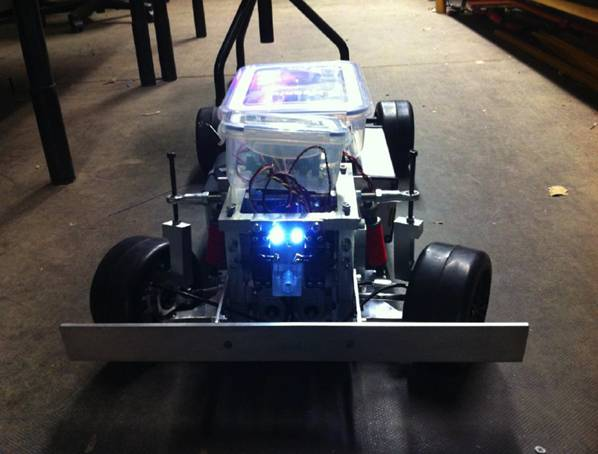
\includegraphics[width=0.7\textwidth]{images/autoedesta}
\caption{Pienoismalli edestä}
\label{fig:autoedesta}
\end{figure}

Elektroniikan puolesta pienoismalli on hyvässä vaiheessa. Anturit ja servot on liitetty mikrokontrollereihin ja aiempien projektiryhmien itserakentamat piirilevytkin on osoittuneet ilmeisen toimiviksi. Aiempana vuotena jarruservoiksi hankitut analogiset servot joudutaan nähtävästi vaihtamaan digitaalisiksi, sillä niiden tarjoama 50Hz päivitysnopeus ei riitä toimivan ABS-järjestelmän toteuttamiseksi. Elektroniikka on kuvassa \ref{fig:elektroniikka}.

Käyttö on toteutettu siten, että jarrualgoritmit yms. toimivat autossa olevilla mikrokontrollereilla, ja ohjaus sekä auton tilan seuranta tapahtuu PC:llä Matlabilla. Tieto Matlabin ja auton välillä kulkee langattomasti XBee-sarjaporttiemulaation yli. Korkean tason rakenne visualisoidaan kuvassa \ref{fig:kommunikointirakenne}.


\begin{figure}[p]
\centering
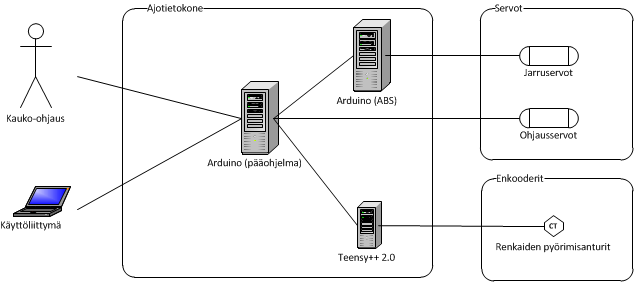
\includegraphics[width=\textwidth]{images/kommunikointirakenne}
\caption{Järjestelmän tämänhetkinen kokonaiskuva}
\label{fig:kommunikointirakenne}
\end{figure}

\begin{figure}[p]
\centering
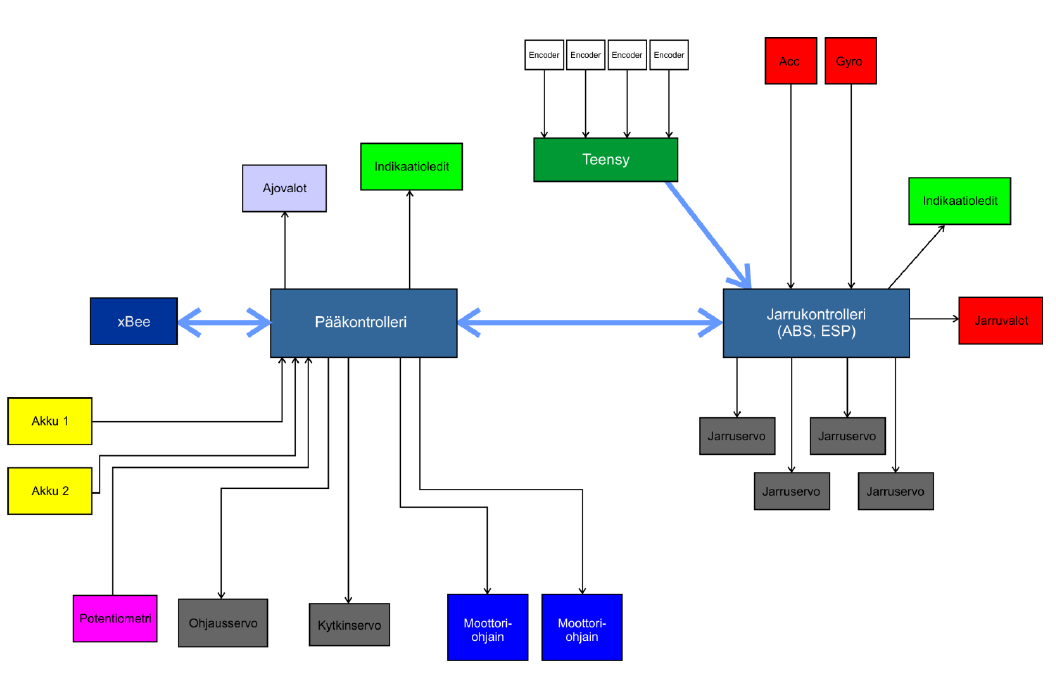
\includegraphics[width=\textwidth]{images/elektroniikka}
\caption{Laitteiston elektroniset kytkennät}
\label{fig:elektroniikka}
\end{figure}

\subsection{Auton koodi ja ohjauselektroniikka}

Autossa on tällä hetkellä kolme mikrokontrolleria suorittamassa erilaisia tehtäviä (kokonaiskuva esitetty kuvassa \ref{fig:elektroniikka}):

\begin{itemize}
	\item Yksi Arduino Mega 2560 pääohjelmalle: kommunikaatio
		käyttöliittymälle, moottoreiden, kytkimen ja valojen ohjaaminen,
		akkujännitteen seuraaminen yms.,
	\item Toinen Arduino Mega 2560 ABS-algoritmille,
	\item Teensy++ 2.0 renkaiden nopeuksien lukemiseen.
\end{itemize}


Toistaiseksi monet eri osat on kytketty näihin kolmeen kontrolleriin kuvan \ref{fig:elektroniikka} mukaisesti. Niitä voidaan kytkeä tarvittaessa uudelleen, mikäli ohjauksen rakenne muuttuu merkittävästi.

Arduino Mega 2560:n ominaisuuksia ovat mm. seuraavat:
\begin{itemize}
	\item 256 KB ohjelmamuistia
	\item 4 KB EEPROMia
	\item 8 KB välimuistia (RAM)
	\item yhteensä 54 i/o-nastaa, joista PWM ja A/D:
	\item 14 näistä nastoista toimii PWM-ulostuloina (esim. servojen ohjaus)
	\item 16 analogista sisääntuloa (jännitemittaus akulta tai antureilta)
	\item 4 UARTia
	\item USB-liitäntä.
\end{itemize}


Teensyn ominaisuuksia:
\begin{itemize}
	\item 128 KB ohjelmamuistia
	\item 4 KB EEPROMia
	\item 8 KB välimuistia
	\item 46 yleistä I/O-nastaa, joista PWM ja A/D:
	\item 9 mahdollista PWM-lähtöä,
	\item 8 analogituloa,
	\item 1 UART,
	\item USB-liitäntä.
\end{itemize}


Tutkitaan, onko tarpeellista käyttää kaikkia kolmea - nykyisellään ohjelma täytyy hajauttaa kolmeen erilliseen osaan, ja ko. mikrokontrollereiden laskentakapasiteetti ei luultavasti tule projektissa esteeksi ja yksi kontrolleri riittäisi ohjaamaan kaikkia servojakin. Ohjausohjelmiston kehitys on helpompaa, jos sitä tarvitsee päivittää vain yhteen kontrolleriin.


\subsection{Käyttöliittymä}


Käyttöliittymä on viime vuoden projektiryhmän päätöksestä toteutettu Matlabin päälle GUIDE-työkalua apuna käyttäen. Käyttöliittymän runko vaikuttaa ensisilmäyksellä toimivalta, joskin koodia joutuu hieman järjestelemään ja kirjoittamaan uudelleen modulaarisemmaksi. Käyttöliittymä näyttää tällä hetkellä tiettyjä auton parametrejä ja auton tilatietoa, mutta suunnitelmissa on lisätä muun muassa akun jännitetieto ja tuoda muutenkin kaikki loput tiedot mikrokontrollereilta ja tallettaa ne lokiin. Käyttöliittymässä on myös kartta auton ajamasta reitistä. Kartta piirretään pelkästään kiihtyvyysanturin tarjoaman datan perusteella, jolloin joudumme integroimaan siihen mukaan myös tiedon renkaiden pyörimisnopeudesta. Automaattiohjausta käyttöliittymään ei ole tällä hetkellä toteutettu.

\begin{figure}[h]
\centering
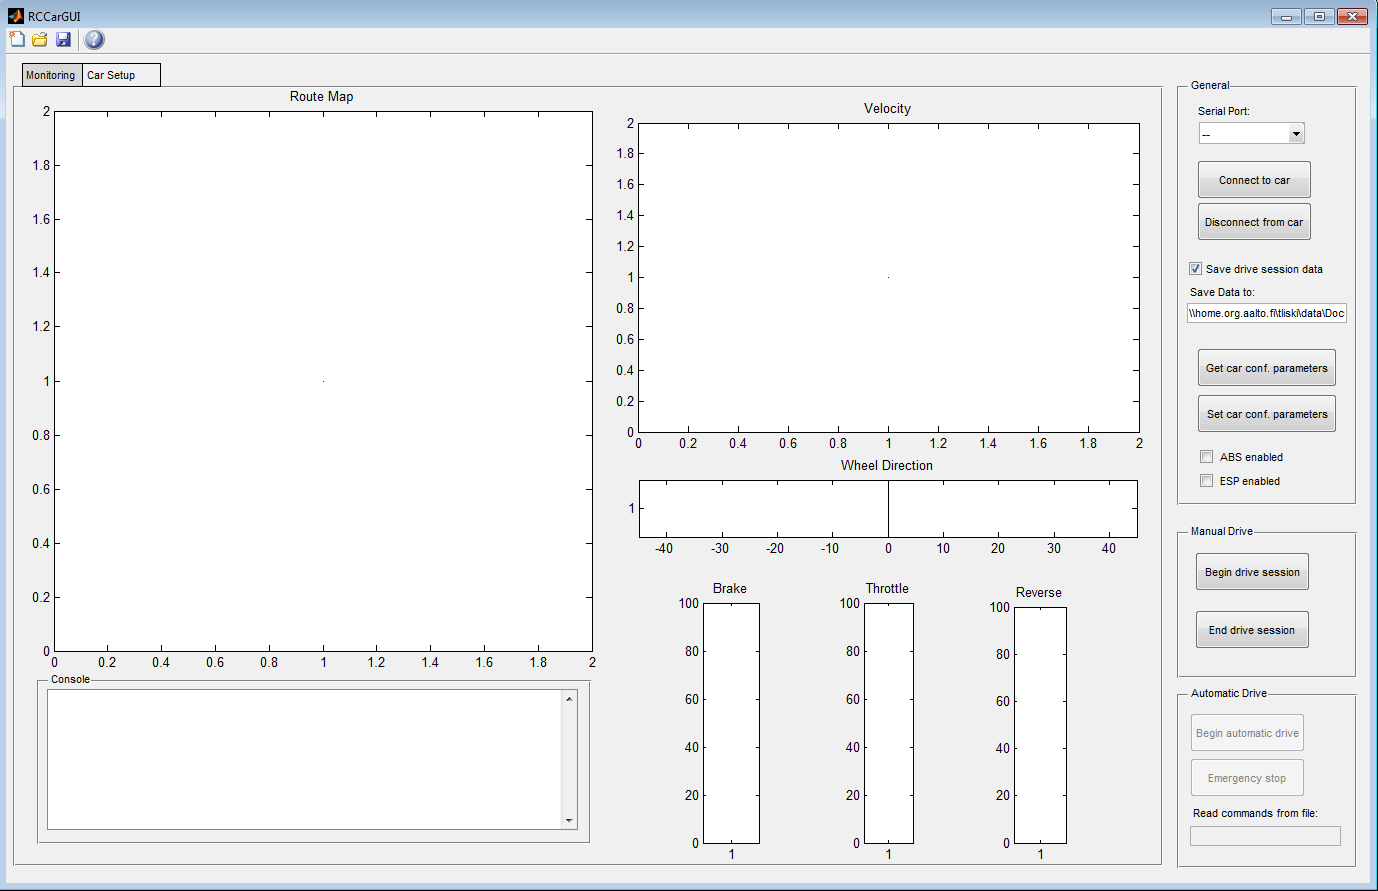
\includegraphics[width=\textwidth]{images/gui1}
\caption{Auton Matlab-käyttöliittymän perusnäkymä}
\label{fig:gui1}
\end{figure}

\begin{figure}[h]
\centering
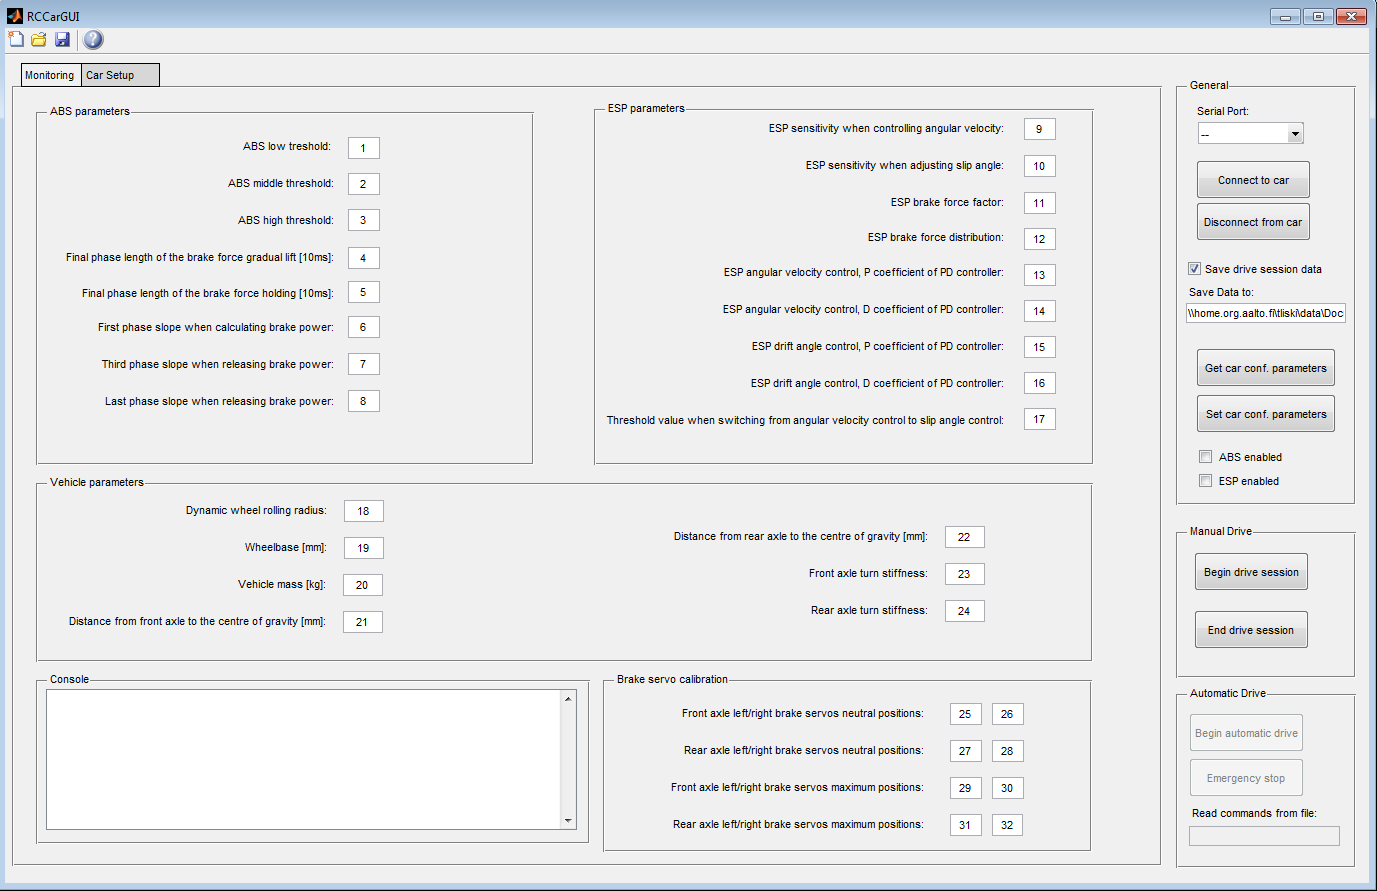
\includegraphics[width=\textwidth]{images/gui2}
\caption{Auton Matlab-käyttöliittymän asetusnäkymä}
\label{fig:gui2}
\end{figure}

\section{Työn rakenne}

\subsection{Vaatimukset}

Jotta ajoneuvon testaaminen ja ajaminen olisi yksinkertaista, tulee siinä olla kauko-ohjaus joko erillisellä ohjaimella tai tietokoneen käyttöliittymän kautta. Edelleen testausta helpottamaan tulee ajoneuvon ohjautua automaattisesti ennaltamääritettyä reittiä pitkin, jolloin esimerkiksi vakioympyrää voidaan ajaa tietokoneen ohjaamana. Ajodynamiikan tutkimista varten käyttöliittymän tulee myös tallentaa ajonaikaista dataa myöhempää käsittelyä varten.

Ajonhallintajärjestelmien (ABS ja ESP) toiminnan tutkimiseksi tulee niiden algoritmien toimia nopeasti ja ennustettavasti.

Kauko-ohjaukseen ja datankeruuseen PC:n puolella tehdään hyvin määritelty kommunikointiprotokolla, jota kummankin pään ohjelmat noudattavat. Protokollan tulee olla helposti laajennettavissa tulevaisuutta varten.

RC-autolle ollaan myös kehittämässä testausympäristöä, missä ajoneuvo ajaa juoksumatosta tehdyllä liukuhihnalla. Testausympäristön toiminnan takaamiseksi tulee paikka liukuhihnalla saada pidettyä vakiona.

Muualla kuin liukuhihnalla ajamisen analysointia varten ajoneuvon paikan seuranta on hyvin tärkeää, ja tämä tullaan toteuttamaan käyttämällä ajoneuvon omia pyörimisnopeus-, kiihtyvyys- sekä gyroanturia. Analysointia tatrvitaan sekä automaattiajoon että datan myöhempään offline-tarkasteluun käsin.

Tällä hetkellä ajoneuvolla ajaminen ei onnistu, koska ajoneuvo pysähtyy välittömästi liikkeellelähdön jälkeen. Pysähtymisen epäillään johtuvan akkujännitteestä, joka käy liian alhaisena ja aiheuttaa akun irtikytkeytymisen akkuvahdin toimesta. Tämän toteamiseksi tulee ajoneuvossa olla akkujännitevahti, mitä pystytään seuraamaan käyttöliittymästä. Mikäli mahdollista, liikkeellelähtöön kiinnitetään ohjauksessa automaattista huomiota siten, että akkujännite ja -virta pysyvät vahdin rajoissa.

\subsection{Lisätavoitteet}

Jos ajoneuvo saadaan sekä käyttöliittymän että ajoneuvon oman ohjelmiston osalta hyvissä ajoin valmiiksi, toteutetaan lisäksi muita ominaisuuksia.

Perustavoitteisiin kuuluu ennalta määriteltyjen reittipisteiden läpi kulkeminen. Tämä pyritään toteuttamaan mahdollisimman luotettavasti niin, että reitti on toistettavissa. Ajan salliessa tehdään esim. helpommin määriteltäviä ratoja käyttäjän kannalta, sekä pyritään ajamaan autoa lähes maksiminopeudella.

Kaikki autossa olevat mittaukset ryömivät hiljalleen, jolloin mittaukseen kasaantuu virhettä, jota on vaikeaa kompensoida. Tätä helpottaisi absoluuttinen paikan mittaus ulkopuolisesta signaalista (kuten GPS tai jokin tarkempi paikallinen kolmiomittaus radiolla) tai ympäristöstä muuten, esim. konenäön avulla.

Kun autoon kiinnitetään etäisyysanturit liukuhihna-ajoa varten joka tapauksessa, niin niitä voi käyttää myös reunan seurantaan: autolle voi rakentaa radan esim. vanerilevyistä, joihin se yrittää pitää sivusuuntaisen etäisyyden vakiona. Radalle voidaan sirotella paikoittain esim. hiekkaa ajonvakautusjärjestelmän testaamiseksi eri pinnoilla automaattisesti.

\subsection{Auton elektroniikka}

Autoon asennetaan ainakin etäisyysanturit ja nopeammat servot jarrujen ohjaukseen.

Etäisyysantureita kytketään yksi kappale eteen liukuhihnalla ajamisen mahdollistamiseksi ja törmäyksen estämiseksi, sekä kaksi toiselle sivulle liukuhihnan sivuttaissuunnan pitämiseksi ja seinän tms. radan seuraamiseksi; kahdella saadaan kulma auton reunan ja seinän välillä, jolloin rattisäädöstä saadaan parempi.

Alkuperäiset jarruservot ottavat ohjausignaalia 50 kertaa sekunnissa, mikä on liian vähän algoritmien kunnollisen toimivuuden takaamiseksi. Pienoismallin mittakaavassa 20 millisekunnin viive säädössä on jo merkittävä yhtään suuremmissa nopeuksissa, mikä lienee syynä siihen, että viime vuoden ryhmä joutui yksinkertaistamaan algoritmiaan. Tutkitaan, korvataanko nykyisten servojen sisäinen ohjauselektroniikka OpenServolla tms, vai ostetaanko koko servojen tilalle nopeat digiservot.

\subsection{Auton ohjelmisto}

Yksi projektin päätavoitteista on helppo jatkokehitys. Auton ohjelmisto (jatkossa “ajotietokone”) on merkittävässä osassa tätä tavoitetta, ja mikäli alkuperäisestä muokkaaminen osoittautuu haastavaksi, ohjelma kirjoitetaan täysin uudelleen vanhan pohjalta. Alkuperäiskoodi on kirjoitettu kokonaan yhteen pötköön ilman varsinaista rakennetta, ja esim. servojen ohjaus on sekoitettu ympäriinsä, mikä hankaloittaa ylläpitoa.

Ajotietokoneen suunniteltu karkea rakenne esitetään kuvassa \ref{fig:software}. Keskeisimpänä suunnitteluaspektina on modulaarisuus ja se, että suuri osa samasta koodista voidaan kääntää tavalliselle PC:lle algoritmien testausta ja simulointia varten; tätä alkuperäinen ohjelma ei salli lainkaan. Tämä laitteistoriippumaton lähtökohta nopeuttaa kehitystä, kun itse auton parissa ei tarvitse istua jatkuvasti testatessa.

Alkuperäinen ohjelma on hajautettu kolmelle kontrollerille siten, että koodia niiden välillä on erityisen hankalaa siirtää paikasta toiseen. Lisäksi servo-ohjaukset, jännitemittaukset ym. piirilevyllä on reititetty siten, että eri kontrollerit suorittavat omia tehtäviään; esimerkiksi rengasenkooderien laskurien siirtäminen pääkontrollerille vaatii uudelleenjohdotusta. Tutkitaan, että vedetäänkö johtoja tiedon ohjelmallisen siirtämisen sijaan: esimerkiksi pääkontrollerissakin riittää pulssisisääntuloja, joten tiedonsiirto-operaatioilta teensyltä pääkontrollerille säästytään, jos kytketään teensylle menevät pulssitulot suoraan sille.

\begin{figure}[H]
\centering
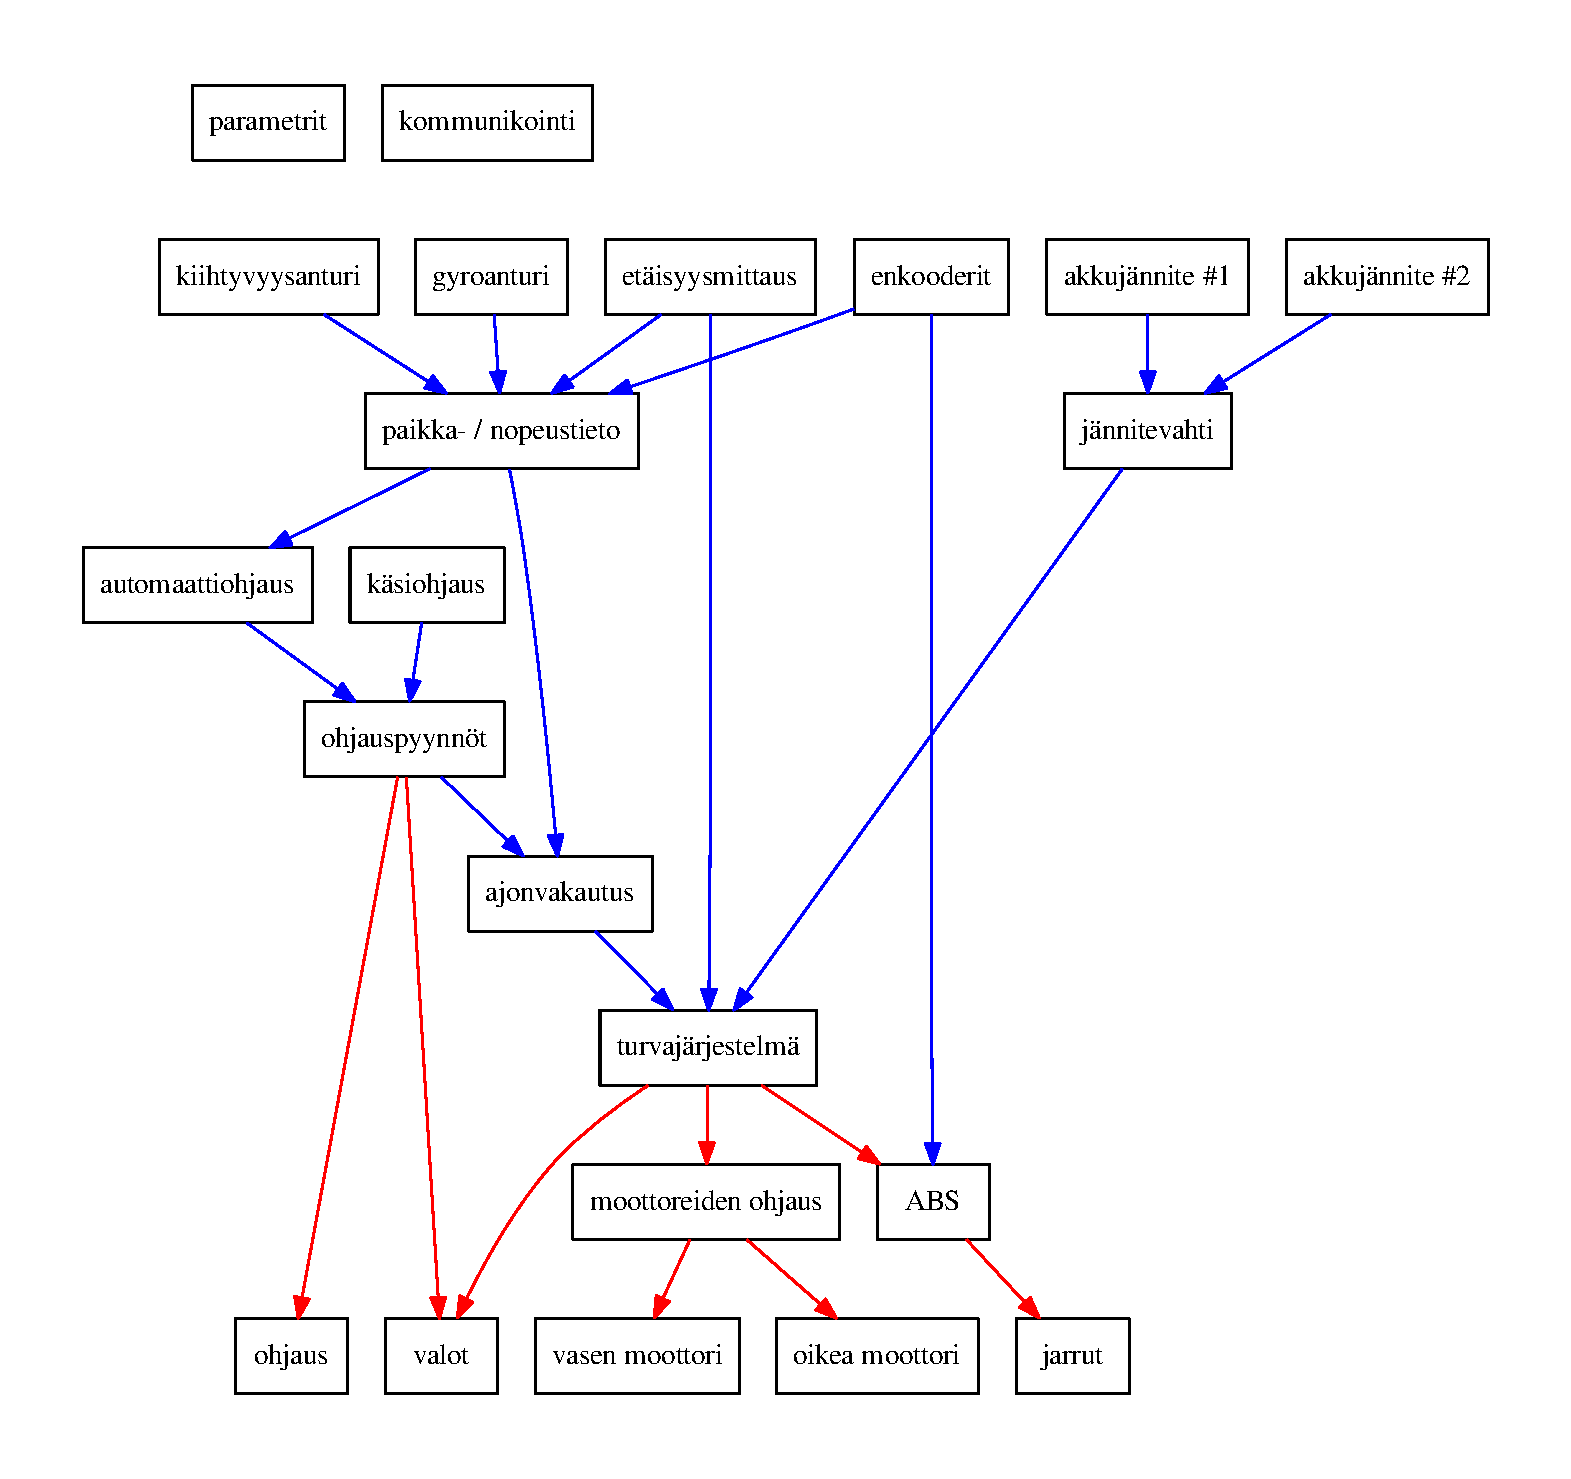
\includegraphics[width=0.7\textwidth]{images/software}
\caption{Alustava suunnitelma ohjelmiston osakomponenteista ja tiedonvälityksestä. Punainen viiva tarkoittaa ohjausta, sininen viiva mittaustietoa.}
\label{fig:software}
\end{figure}

Kommunikointikoodi kehitetään siirtämään paketteja dataa autosta ja autolle (kuten ajonopeus, servoparametrit, tavoitenopeus tai ratin suunta) niin, että pakettien hallinta on riippumaton muusta koodista. Näin toimimalla suunnittelemattoman datan siirron lisääminen on triviaalia.

Automaattiohjaus toimii reittipistepohjaisesti. Aluksi tehdään vain yksinkertainen pisteestä pisteeseen -ajo, jossa auto pyrkii pitämään tasaisen (ja turvallisen hitaan) nopeuden, sekä suunnan seuraavaan pisteeseen. Auton kinematiikan vuoksi pisteille pitänee määrittää myös auton suuntakulma maailmakoordinaatiston suhteen. Ajan salliessa ajetaan suorien viivojen sijaan kaarissa, jotka määritellään jo käyttöliittymässä. Radiolinkin latenssi käyttöliittymältä autolle ei tule ongelmaksi hitaissa nopeuksissa, joten automaattiohjaus kehitetään Matlab-koodina, josta kirjoitetaan myöhemmin ohjauskoodi itse autolle.

Koska auton mittausjärjestelmät ovat ryömivää luonnetta, reittipisteohjausta ei luultavasti tulla käyttämään kovin pitkillä reiteillä. Paikan integrointi kiihtyvyysantureilta ei ole sataprosenttisen tarkkaa, ja renkaatkin saattavat lipsua eikä niiden ympärysmitta ole tarkka. Paikka- ja nopeustietoa voidaan lukea sekä renkaista että kiihtyvyysanturista sekä kaikissa on omat virhelähteensä yms, joten ne yhdistetään Kalman-filtterillä.

Ajotietokoneelle tehdään prioriteettipohjainen tehtävänhallinta (skedulointi) siten, että säätimet pysyvät jatkuvasti ajan tasalla ja datan keruu käyttöliittymälle menee puskurin kautta, jota siirretään kun ehditään. Kun sarjaportilta tulee ohjausdataa käyttöliittymältä, sitäkin puskuroidaan kunnes sen hallinnalle on aikaa. Kriittisimmät ohjaukset suoritetaan keskeytyksillä.

Toimilaitteiden ohjaus toteutetaan hierarkisesti: automaatti- tai manuaaliohjaus syöttää moottoreille kohdenopeutta, johon toivottaisiin päästävän. Syystä tai toisesta moottoreita ei silti välttämättä pystytä ohjaamaan tavoitesignaalilla: edessä saattaa olla seinä (mitataan keulan etäisyysanturilta), tai voimansiirron aiheuttama hitaus voi rajoittaa ohjaussignaalin muutosnopeutta (esim. täydessä vauhdissa ei kannata laittaa pakkia päälle). ESP rajoittaa ohjausliikkeitä vielä entisestään (mm. luistonesto) tämän turvakerroksen päällä.

\subsection{Matlab-käyttöliittymä}

Edellinen ryhmä oli toteuttanut käyttöliittymän Matlabiin käyttäen apuna GUIDE-käyttöliittymänsuunnittelu-työkalua. Työkalu generoi käyttöliittymän taustalla olevat tynkä-funktiot automaattisesti yhteen tiedostoon, jolloin suunnittelematta koodin rakennetta kummemmin, koko toiminnallisuus voi äkkiarvaamatta rakentua yhteen 2000-riviseen kooditiedostoon, kuten viime kerralla näytti käyneen. Kuvassa \ref{fig:origsofta} on vanhan ryhmän rakennekaavio Matlabilla pyörivästä ohjelmistosta. Tarkoituksemme on jakaa koodi (kuvassa “taustakoodi”) modulaarisempiin lohkoihin ja selkeyttää rakennetta muutenkin. Tarkoituksena on myös kommentoida koodia siten, että sen työstäminen jälkikäteen helpottuu.

\begin{figure}[H]
\centering
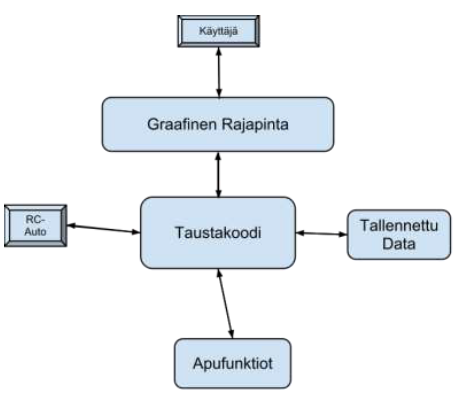
\includegraphics[width=0.6\textwidth]{images/origsofta}
\caption{Viimevuotisen ryhmän näkemys käyttöliittymän rakenteesta}
\label{fig:origsofta}
\end{figure}

\subsection{Simulointi ja testaaminen}

Varsinaisen ajotietokoneen simulointi tapahtuu siten, että esim. Matlabilla tuotetaan todenmukaisen oloista anturidataa, jonka perusteella ajetaan ohjaustietokoneen simulointiversiota PC:llä säätäen moottoreita ja jarruja. Säätösignaalit ja auton parametrit otetaan talteen ja analysoidaan Matlabilla. ABS:n simuloinnissa käytetään hyödyksi viime vuoden projektin Matlab-malleja.

Simulointiohjelma on muunneltu versio ajotietokoneesta, jossa varsinaisten oheislaitteiden mittaaminen ja “ohjaus” suoritetaan esimerkiksi tiedostojen kautta. Itse algoritmit ja kommunikointikoodi pyritään pitämään mahdollisimman paljon muuttumattomana siitä, millaisena se käännetään itse auton kontrollereille. Enimmäkseen ajotietokonetta tullaan ohjaamaan Matlab-käyttöliittymän kautta, mutta yksikkötestejä varten simulaatiokoodille kirjoitetaan automaattiskriptejä erinäisillä muillakin työkaluilla.

Algoritmien laskentatehokkuutta voi testata ajamalla käännettyä avr-koodia simulaattorissa esim. AVR Studiossa, joka mittaa suoritukseen kuluvat käskyt. Tätäkin testausta hyödyttää se, että koodin jakaa irrallisiin palasiin, joista vain algoritmin voi helposti irrottaa ja testata ennaltamäärätyllä syötteellä.

Testausta tehdään autolla sitten, kun ohjelma ja auton mekaniikka ovat siinä vaiheessa, että autolla voi ajaa. Energiankulutusta, moottorien ohjausta yms. pyritään kokeilemaan liukuhihnalla, jossa auto voi pysyä paikallaan työpajassa. Viime vuoden ryhmän jälkiä seuraamalla ABS-jarruja voidaan kokeilla aluksi pyörittämällä pyöriä momenttisäätöisellä akkuporakoneella. Kokonaisjärjestelmää on luonnollisesti selkeintä testata ajamalla autolla ulkotiloissa runsaasti jarrutellen ja mutkitellen. Kun auto lähettää ohjaus- ja mittausdatat jatkuvasti käyttöliittymälle, niitä voidaan verrata ennustettuihin tuloksiin bugien metsästämiseksi.

\section{Ajanhallinta ja tehtävien jakautuminen}

\subsection{Työn osa-alueet}

Työ jakautuu karkeasti seuraaviin osa-alueisiin:

\begin{itemize}
	\item Olemassaolevan ympäristön kartoitus
	\item Mekaniikan kehitystyö
	\item Auton ohjelmiston kehitystyö
	\item Käyttöliittymän kehitystyö
\end{itemize}

Työ alkaa luonnollisesti kartoittamalla jo olemassaolevan RC-auton järjestelmiä, elektroniikkaa, ohjelmistoja ja käyttöliittymää. Kartoitus sisältää koodien opiskelua ja dokumentaatioon perehtymistä.

Mekaniikan kehitystä voidaan tehdä samanaikaisesti ohjelmistoa koodatessa. Analogiset jarruservot vaihdetaan nopeammiksi ja autoon lisätään etäisyysanturit. Tämä työ sisältää laitteiston valinnan, tilaamisen ja asentamisen, mikä vie aikaa. Koodi on kuitenkin riippumaton tämän vaiheen tilasta, ja mekaniikkatiimin mukaan autolla ei muutenkaan päästä ajamaan kovaa vielä hetkeen. Pyritään siis etenemään mahdollisimman pitkälle simuloimalla.

Auton varsinainen kehitys eli ohjelmistopuolen jatkokehitys alkaa hyvissä ajoin olemassaolevien järjestelmien kartoituksen jälkeen. Tämä vaihe pitää sisällään auton mikrokontrollereiden ohjelmistoon tehtävät muutokset ja päivitykset, kuten jarrualgoritmin kunnostuksen ja ajoneuvonvakautusjärjestelmän käyttöönoton, sekä mahdollisen koko koodin uudelleenjärjestelyn.

Listan neljäs vaihe on Matlab-käyttöliittymän kehitys, ja samalla kommunikaatioväylien uudelleenmäärittely ja tarkka dokumentointi. Käyttöliittymään lisätään myös kaikki loput auton parametrit ja niiden tallennus, sekä automaattiajo ennaltamääriteltyjen reittipisteiden kautta. Neljäs vaihe voidaan suorittaa muiden vaiheiden kanssa samanaikaisesti, koska siihen liittyvät tehtävät eivät riipu muista vaiheista.

Taulukossa \ref{fig:osaalueet} on eritelty projektin osa-alueet tarkemmin ja arvioitu jokaiselle osa-alueelle summittainen työmäärä.


\begin{figure}
	\begin{tabular}{l l l l l}
		No. & Tehtävä & Vastuu & Riippuu teht. & Työmäärä (h) \\
		\hline
		1 & Jarruservojen tilaus ja vaihto & Konsta, Lasse & 4 \\
		2 & Etäisyysantureiden tilaus ja asentaminen & Konsta, Lasse & 5\\
		3 & Koodeihin tutustuminen & Kaikki & 5\\
		4 & Dokumentteihin tutustuminen & Kaikki & 3\\
		5 & Autoon tutustuminen & Kaikki & 3\\
		6 & ABS-algoritmi & Lasse & 10\\
		7 & ESP-algoritmi & Lasse & 10 \\
		8 & Ajotietokoneen skeduleri ja kehyskoodi & Konsta & 12 \\
		9 & Kommunikaatiokoodin tulkinta & Toni, Konsta & 2 \\
		10 & Kommunikaatioprotokollan määrittely/muutokset & Toni, Konsta & 9 & 6 \\
		11 & Kalman-filtteri paikan mittaukseen & Konsta & 12 \\
		12 & Kauko-ohjauksen toteutus & Konsta, Toni & 8 \\
		13 & Auton Simulink-mallin luominen & Lasse, Konsta & 8 \\
		14 & Auton mallin parametrien mittaaminen & Lasse, Konsta & 4 \\
		15 & Käyttöliittymäkoodin kehittäminen & Toni & 10 \\
		16 & Kaikkien mittaustietojen tuonti käyttöliittymään & Toni & 10 & 3 \\
		17 & Auton paikan päivitys käyttöliittymään & Toni & 16 & 3 \\
		18 & Mittausdatan tallentaminen & Toni & 16 & 2 \\
		19 & Automaattiajo reittipisteiden kautta & Toni, Konsta & 17 & 12 \\
		20 & Automaattiajon lopputestaus ja muutokset & Toni, Konsta & 11, 19 & 5 \\
		21 & ABS:n lopputestaus & Lasse & 1, 6 & 3 \\
		22 & ESP:n lopputestaus & Lasse & 1, 7 & 3\\
		23 & Kauko-ohjauksen lopputestaus & Konsta, Toni & 12 & 3 \\
		24 & Käyttöliittymän lopputestaus & Toni & 19 & 3 \\
	\end{tabular}
	\label{fig:osaalueet}
	\caption{Projektin osa-alueet, niiden vastuuhenkilöt, riippuvuudet ja arvioidut työmäärät.}
\end{figure}

Tavoite: (näitä ei välttis dokkariin…)

Toni: ~70h ~3op

Lasse: ~100h ~4op

Konsta: ~130h ~5op

\subsection{Ajankäyttöarvio ja aikataulutus}

Alkuperäisen projektikuvauksen mukaan työstä oli tarkoitus saada 4 opintopistettä per henkilö. Työ oli lisäksi tarkoitettu vain kahdelle henkilölle. Nyt ryhmässämme on kolme henkilöä, mutta työtä kuulemma riittää niin paljon kun halutaan, eli kaikille todennäköisesti riittää tekemistä. Opintopisteiden suhteen lähdetään liikkeelle siitä, että Konsta olisi ottamassa projektista muita vähän suuremman osan, siten että hänen osuutensa vastaisi suurin piirtein 5 opintopistettä. Lasselle pyritään jakamaan noin 4 opintopisteen suuruinen osuus ja Tonille 3 opintopistettä.

Työn jakaminen pyritään tasapainottamaan siten, että kaikilla on jatkuvasti vahva yleiskuva projektista ja pyrimme tekemään paljon asioita yhdessä. Tällöin kuka tahansa voi jatkaa jotain osa-aluetta, joka osoittautuu muita työläämmäksi.

Osa-alueiden työmääräarvioista voidaan laskea jokaiselle oma kurssin työmäärä. Osa-alueissa ei ole otettu huomioon luentoihin, esityksiin ja dokumentointiin kuluvaa aikaa.

Taulukossa \ref{fig:aikataulu} on esitettynä tehtävien suunniteltu aikataulutus. Perustoiminnallisuudet pyritään saamaan toimivaksi aikaisessa vaiheessa; lopuksi keskitytään varsinaiseen ajodatan analysointiin ja säätöön, mikä tarvitsee toimivan ja luotettavan pohjakoodin.

\begin{figure}[H]
	\begin{tabular}{l|l|l|l|l|l|l|l|l|l|l|l|}
		Tehtävä \\
		\hline

		Jarruservojen vaihto
		&   &   & x & x &   &   &   &   &   &   &   \\
		Etäisyysantureiden asentaminen
		&   &   & x & x &   &   &   &   &   &   &   \\
		Koodeihin tutustuminen
		& x & x & x &   &   &   &   &   &   &   &   \\
		Dokumentteihin tutustuminen
		& x & x & x &   &   &   &   &   &   &   &   \\
		Autoon tutustuminen
		& x & x & x &   &   &   &   &   &   &   &   \\
		Ajonvakautusalgoritmien opiskelu
		& x & x & x &   &   &   &   &   &   &   &   \\
		Ajotietokoneen kehyskoodin hahmottelu
		&   & x & x & x &   &   &   &   &   &   &   \\
		Kommunikointiprotokollan määrittely
		&   &   &   & x & x &   &   &   &   &   &   \\
		Kommunikoinnin ja kauko-ohjauksen perustoteutus
		&   &   &   &   & x & x & x &   &   &   &   \\
		Simulointiympäristön toteutus ja ensitestaus
		&   &   &   & x & x & x &   &   &   &   &   \\
		Auton parametrien mittaus simulointia varten
		&   &   &   & x & x &   &   &   &   &   &   \\
		Kehyskoodin käyttö oheislaitteiden ohjaukseen
		&   &   &   & x & x &   &   &   &   &   &   \\
		Servojen parametrien etsintä
		&   &   &   &   & x & x &   &   &   &   &   \\
		Testiajo perustoiminnallisuuksilla
		&   &   &   &   & x & x &   &   &   &   &   \\
		Auton mittausdatan simuloinnin kehitys
		&   &   &   &   & x & x &   &   &   &   &   \\
		Paikkaseuranta käyttöliittymään
		&   &   &   &   & x & x & x &   &   &   &   \\
		Kaiken mittausdatan tuonti käyttöliittymään
		&   &   & x & x & x &   &   &   &   &   &   \\
		Auton datan ja parametrien tallennuksen kehitys
		&   &   & x & x & x &   &   &   &   &   &   \\
		Kalman-filtteri paikkamittaukseen
		&   &   &   &   &   & x & x & x &   &   &   \\
		Turvajärjestelmien toteutus 
		&   &   &   &   & x & x & x &   &   &   &   \\
		ABS-järjestelmän toteutus
		&   &   & x & x & x &   &   &   &   &   &   \\
		ABS-järjestelmän testaus ja ruuvaus
		&   &   &   &   & x & x & x &   &   &   &   \\
		ESC:n toteutus
		&   &   & x & x & x &   &   &   &   &   &   \\
		ESC:n testaus ja säätö
		&   &   &   &   & x & x & x &   &   &   &   \\
		Automaattiajon perusrakenne
		&   &   &   &   &   & x & x & x &   &   &   \\
		Tehokas automaattiajo
		&   &   &   &   &   &   &   & x & x & x &   \\
		Kauko-ohjaus joystickillä
		&   &   &   &   &   &   &   & x & x &   &   \\
		Kaikenkattava testaus
		&   &   &   &   &   &   &   &   &   & x & x  \\

		\hline
		Viikko & 38 & 39 & 40 & 41 & 42 & 43 & 44 & 45 & 46 & 47 & 48
	\end{tabular}
	\label{fig:aikataulu}
	\caption{Taulukko 2: Projektin osa-alueiden aikataulusuunnitelma.}
\end{figure}

\section{Riskienhallinta}

RC-auton piti olla valmis jo syksyllä 2012, mutta voimansiirrossa ilmenneistä ongelmista johtuen tänä syksynä uusitaan sekä moottorit että tasauspyörästö. Tästä johtuen testaaminen lopullisella mekaniikalla siirtyy aivan projektin loppuun; alkuperäisellä voimansiirrolla voidaan ajaa vain lyhyitä kokeita. Ettei ohjelmiston testaus riippuisi valmiista ajoneuvosta, tullaan sitä testaamaan simuloimalla. Viime syksyn ryhmä kuitenkin onnistui ajamaan autoa (joskin hitaasti), joten suurempia ongelmia ei ole odotettavissa.

Mikrokontrollerien laskentateho on rajallinen. Jos yhden laskenta-aika ei riitä sekä ABS- että ESP-algoritmien ja muun oheisen pyörittämiseen, voidaan pyrkiä hajauttamaan laskentaa, kuten on jo tehty: kontrollereita on kolme, joista kukin suorittaa omaa tehtäväänsä. Ohjelman modulaarinen rakenne mahdollistaa sen, että eri algoritmit voidaan tarvittaessa siirtää eri suorittimille helposti.

Rajallisesta budjetista johtuen hankinnat joudutaan tekemään ulkomaisista nettikaupoista, mikä tuo painetta tehdä hankintapäätökset nopeasti. Budjettimme on yhdistetty mekaniikkatiimiin, joten voimansiirrossa ilmenevät mahdolliset yllättävät kustannukset siirtyvät meillekin. Suuri osa viime vuoden ohjauksen mekatroniikasta on kuitenkin käytettävissä. Kun tarvittavat osat määritellään varovaisesti heti aluksi, säästytään siltä riskiltä, että tilatut osat eivät kelpaakaan.

Ohjausjärjestelmän kompleksisuuden hallinnaksi projektia kehitetään iteratiivisesti ja tilannetta tarkastellen. Eri osasten välinen riippuvuus pyritään minimoimaan.

Suunnitelmaan kuuluu säätöalgoritmien prototyyppien testaaminen Matlabilla radiolinkin ylitse. Tässä kommunikoinnissa tulee väistämättä pientä viivettä, mikä vaikuttaa säätöön. Mitataan ja analysoidaan viiveet siten, että algoritmi ottaa ne huomioon, mikäli ne osoittautuvat merkittäviksi asian suhteen.

Aikataulun venymisen riskejä hallitaan limittämällä työskentelyä, ja työstämällä eri osia itsenäisesti. Rakennetaan simulointiympäristö niin, että keskeneräiset osa-alueet voidaan korvata tyhjillä implementaatioilla, jotka toteuttavat vain minimaaliset ominaisuudet. Näin riippuvuus eri töiden välillä ei haitanne.


\end{document}
